\chapter{Retrieval, Grounded Generation and Agent Design}
\label{ch:agent}
\minitoc

\section*{Introduction}
\addcontentsline{toc}{section}{Introduction}
The facts are stored in the knowledge graph. This chapter explains the layer that converts a typed and/or spoken query into an answer from it. These are three problems that need to be solved in order: figuring out what the user is talking about, figuring out what he wants to know about it, and saying it back to him in a way that doesn't go against the grain of the situation.

The third is the place the majority of design work went, which sets this system apart from the typical retrieval-augmented assistant\citep{lewis2020rag}. This language model is not relied on to make any decisions. It is fed facts it has already retrieved and can only be asked to restate them; no results are presented until it confirms what it has said with the facts.

\section{Retrieval Methodology}

Resolving what a question is about comes before anything can be said about it, and the
system takes two different routes depending on how the question is phrased: a fast,
unambiguous path for a question naming an identifier directly, and a ranked free-text path
for everything else. Both routes are described below, along with the numeric gates that
decide what a free-text score is allowed to become.

\subsection{Identifier Fast Path}

If a question has something in it that looks like an activity identifier, it first attempts a direct look-up. Identifiers are unique, so there is no ambiguity and a match is precise. This route is the low cost route, and it's the one that is used by those users who already know what they're looking for.

If an identifier is not found in the node set, it is considered as a different result and not as a failure. This distinction is not as insignificant as it may seem. Previously, an unrecognised identifier would be matched with free text search over the entire question, including the bogus identifier itself. The other words of the question (such as ``task'', ``who'', and ``approves'') have enough common vocabulary with real activity titles to score positive, but would have been confused with the actual activity a user was asking about. The behaviour was not an edge case situation, but a natural case.

\subsection{Identifier Grammar and the Invalid-Identifier Branch}
\label{sec:idgrammar}

An identifier is recognised by the pattern
\texttt{\textbackslash d+(\textbackslash.\textbackslash d+)\{1,3\}(\textbackslash.[a-z])?},
which admits between two and four dotted numeric components and an optional trailing letter.
It therefore matches \texttt{2.126}, \texttt{1.117.2}, \texttt{2.432.4.a} and rejects a bare
integer, so an ordinary monetary figure in a question is not mistaken for an activity
reference.

Recognition and existence are separate tests, and the separation produces three outcomes
rather than two. A matched string that is a key in the node set resolves immediately at
confidence $1.0$. A matched string that is not a key routes to a distinct
\texttt{invalid\_id} outcome. A query containing no identifier-shaped substring at all falls
through to the free-text path.

The middle outcome exists because merging it into free-text search produces a specific
failure. A question such as ``who approves 9.999.999'' still contains the words
\emph{who} and \emph{approves}, and those words alone are sufficient to score against some
unrelated real activity. The system would then answer confidently about an activity the user
never named. Routing the case separately means the response states that the identifier does
not exist.

Suggestions accompanying that refusal are computed by longest shared dotted prefix. For an
invalid identifier $x$, every indexed node whose leading component equals that of $x$ is
ranked by

\[
\operatorname{depth}(x, n) \;=\; \max \{\, j : x_{1..j} = n_{1..j} \,\},
\]

the number of leading dotted components the two share, and the three highest are returned.
If the leading component itself matches no node, the identifier is stripped from the query
and the remaining words are put through the text index instead, so a malformed reference
accompanied by a usable description still yields candidates.

\begin{figure}[htbp]
\centering
% ---------------------------------------------------------------
% PLACEHOLDER — replace with a flow diagram of the resolution path:
%   query -> identifier regex match?
%        yes -> exists in node set? -> resolve (score 1.0)
%                                   -> invalid_id + prefix suggestions
%        no  -> typo correction -> TF-IDF -> threshold gate
%                -> answer / clarify / refuse
% Suggested filename: figures/fig5_resolution_flow.png
% ---------------------------------------------------------------
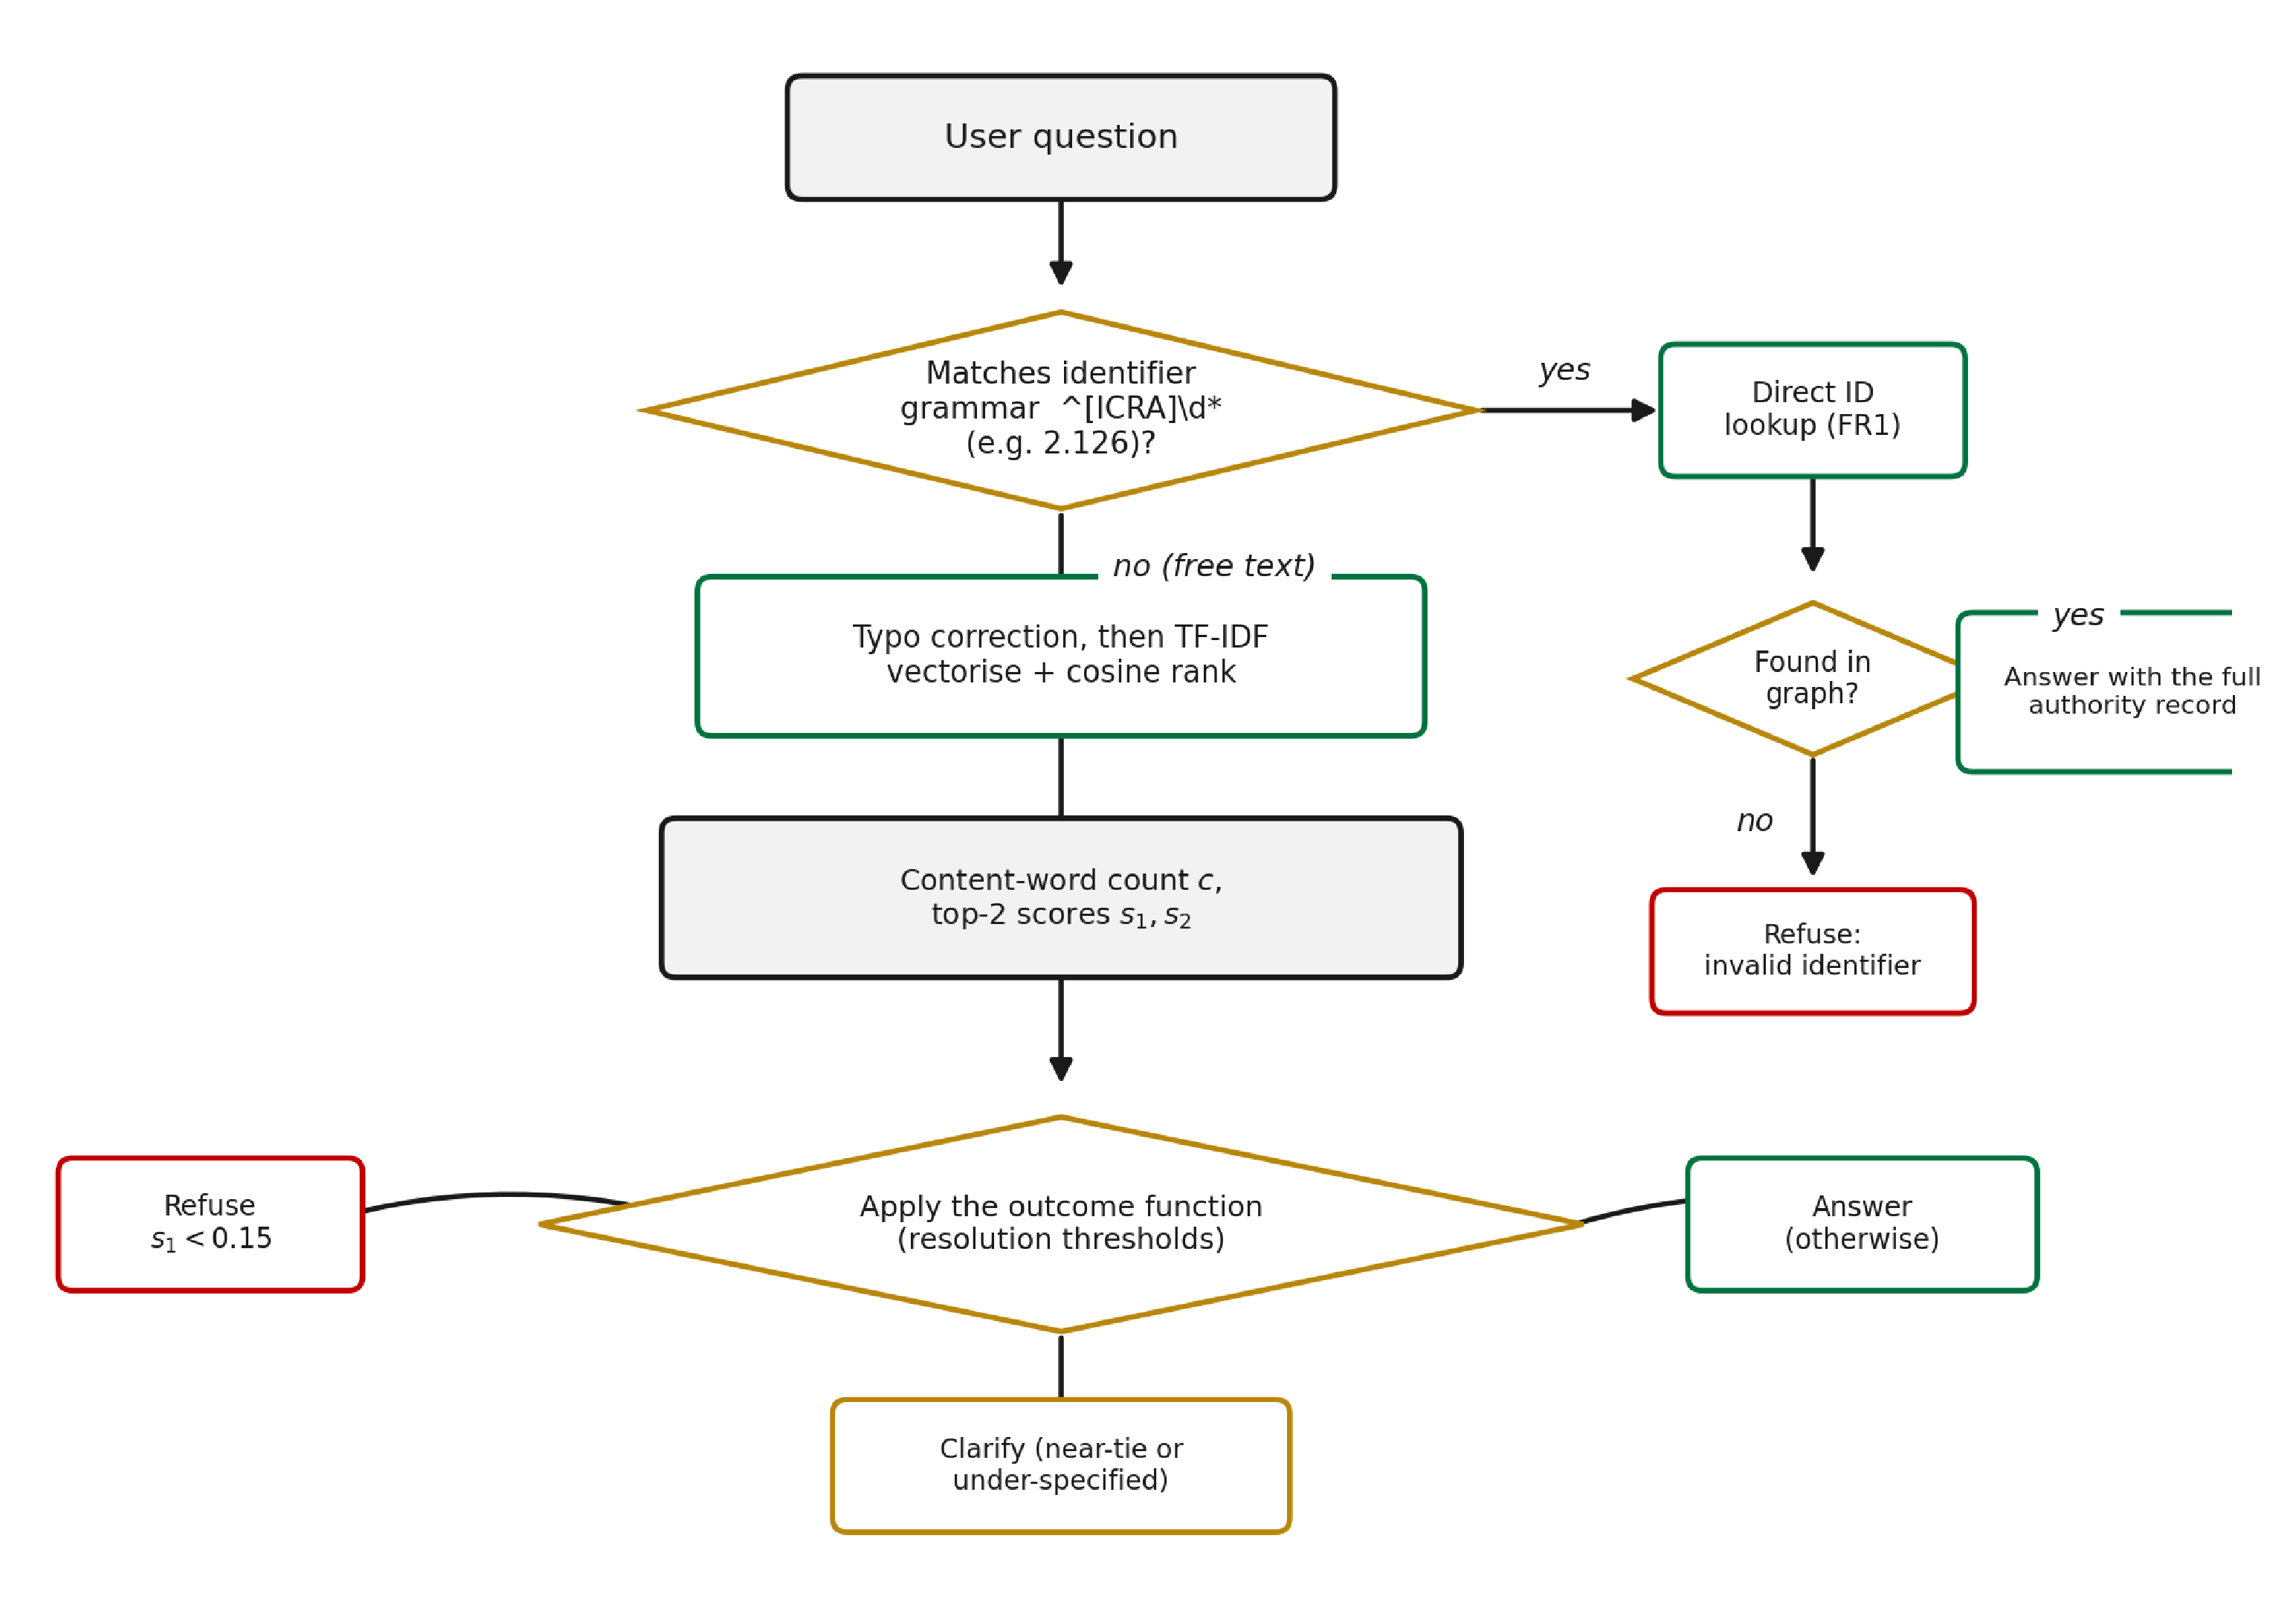
\includegraphics[width=0.9\textwidth]{figures/fig5_resolution_flow.pdf}
\caption{Resolution decision flow, from raw query to one of four outcomes: identifier
resolution, invalid-identifier refusal, clarification, or a scored free-text match.}
\label{fig:resolutionflow}
\end{figure}

Figure~\ref{fig:resolutionflow} shows the complete path, including the threshold gate
described in Section~\ref{sec:confidence}.

\subsection{Free-Text Resolution}

If the question mentions an activity but not any specific activity, lexical similarity is used to resolve the question. Each activity is represented in a vector using TF-IDF\citep{salton1988,manning2008ir} and a comparison is performed to the question by cosine similarity, returning the vector with the highest score and its value.

Tasks and child tasks, as well as process-level titles, are included in the index. Initially they were excluded because they didn't ask about activities, they asked about grouping organisations. The user was asking about the organisation of missions in the non-sovereign chapter, and so he was seeking to match nothing useful, since the only node with a title that had that phrasing was a process, and processes were not indexed.

\subsection{Index Construction}
\label{sec:indexconstruction}

The free-text path is served by a TF-IDF index\citep{salton1988,manning2008ir} fitted once at
startup and held in memory for the lifetime of the process. Table~\ref{tab:indexparams} gives
its configuration.

\begin{longtable}{|p{0.26\textwidth}|p{0.22\textwidth}|p{0.42\textwidth}|}
\caption{Configuration of the TF-IDF retrieval index.}\label{tab:indexparams}\\
\hline
\rowcolor{myblue}\textcolor{white}{\textbf{Parameter}} & \textcolor{white}{\textbf{Value}} & \textcolor{white}{\textbf{Effect}} \\
\hline
\endfirsthead
\hline
\rowcolor{myblue}\textcolor{white}{\textbf{Parameter}} & \textcolor{white}{\textbf{Value}} & \textcolor{white}{\textbf{Effect}} \\
\hline
\endhead
Corpus unit & Activity title & One document per indexed node; the title is the only field vectorised. \\ \hline
Indexed node types & \texttt{process}, \texttt{task}, \texttt{child\_task}, \texttt{threshold\_variant} & Chapter nodes are excluded, since chapter titles are empty in the extracted set. \\ \hline
Empty-title filter & applied & A node whose title is blank after normalisation contributes no row. \\ \hline
\texttt{stop\_words} & \texttt{"english"} & Removes closed-class English words before weighting, so shared function words do not raise a score. \\ \hline
\texttt{ngram\_range} & $(1,2)$ & Indexes unigrams and bigrams. A two-word phrase such as ``mission programme'' contributes a term of its own in addition to its parts. \\ \hline
Similarity & Cosine & Scores lie in $[0,1]$; $0$ means the query and title share no weighted term. \\ \hline
Candidates returned & $k = 5$ & The ranked list the resolution layer receives. Zero-scoring rows are discarded before return. \\ \hline
Mutability & Read-only after fit & The matrix is never refitted at runtime, so an identical query returns an identical ranking for the life of the deployment. \\ \hline
\end{longtable}

Including bigrams matters for this corpus because DAM titles are short noun phrases in which
word order carries meaning. ``Report to the Board'' and ``Board report'' share every unigram
and no bigram, and a unigram-only index scores them identically.

Given a query $q$ and the set of indexed titles $D$, the resolved candidate set is

\[
R(q) \;=\; \operatorname*{arg\,top-}_{d \in D}{}^{k}\;
\frac{\mathbf{v}(q)\cdot\mathbf{v}(d)}{\lVert \mathbf{v}(q)\rVert\,\lVert \mathbf{v}(d)\rVert},
\qquad k = 5,
\]

where $\mathbf{v}(\cdot)$ is the TF-IDF transform described above. The score is lexical
overlap. A score of $0$ states that the query shares no weighted term with the title, which
is not the same claim as the activity being unrelated to the question.

\subsection{Why Lexical Retrieval Rather Than Embeddings}

The more popular solution is semantic retrieval using learned embeddings – this is the one that would apply to a large and diverse body of ordinary language text. The volume of this corpus is not large and it is not representative. It's a handful of hundred short papers that have been expressed in a specific institutional jargon, such that the words the user will type are the ones most likely used by the document.\\[0.3cm]
Lexical matching is also explainable: this is a property that is important for this project. The shared terms can be carried as a score, a mismatch can be identified by analyzing the vocabulary, and the entire layer runs without downloading a model, without an inference cost, and without relying on an external service. As retrieval accuracy was the key for everything else, it was more valuable to be able to reason about why a given node was returned than to get the additional recall that an embedding model might have provided.

\subsection{Typo Tolerance}

People misspell things, particularly long institutional phrases. Rather than relying on a language model to interpret intent, the system applies a deterministic correction step: each alphabetic word in the question is compared against the vocabulary the document itself uses, and replaced with the closest match when the similarity exceeds a threshold and the word is not already an exact match.

The threshold was calibrated against a real false positive rather than chosen by intuition. Set too low, ordinary words get rewritten into document vocabulary they merely resemble, which corrupts questions that were correct to begin with. Because the step is deterministic, it behaves identically whether or not a language model provider is reachable.

\subsection{Correction Algorithm and Parameters}
\label{sec:typoparams}

Correction runs before vectorisation and operates on the query alone; the index is never
altered. Each alphabetic token is compared against the vocabulary of single words the
vectoriser already holds, so the correction target is the document's own wording rather than
a general English dictionary. A token identical to a vocabulary entry under case folding is
left alone. Otherwise the closest vocabulary entry is retrieved by Ratcliff--Obershelp
sequence matching, and the token is replaced only when that similarity reaches the threshold
in Table~\ref{tab:typoparams}. A token with no sufficiently close match is passed through
exactly as typed.

\begin{longtable}{|p{0.27\textwidth}|p{0.17\textwidth}|p{0.46\textwidth}|}
\caption{Parameters governing deterministic typo correction.}\label{tab:typoparams}\\
\hline
\rowcolor{myblue}\textcolor{white}{\textbf{Parameter}} & \textcolor{white}{\textbf{Value}} & \textcolor{white}{\textbf{Effect}} \\
\hline
\endfirsthead
\hline
\rowcolor{myblue}\textcolor{white}{\textbf{Parameter}} & \textcolor{white}{\textbf{Value}} & \textcolor{white}{\textbf{Effect}} \\
\hline
\endhead
Similarity measure & Ratcliff--Obershelp ratio & Length-normalised, in $[0,1]$. Computed against the index vocabulary, not an external dictionary. \\ \hline
Acceptance threshold & $0.88$ & A token is replaced only at or above this similarity. Below it, the token is left as typed. \\ \hline
Minimum token length & $4$ characters & Tokens of three characters or fewer are skipped entirely. \\ \hline
All-capital tokens & Skipped & A fully capitalised token is treated as an institutional acronym and never corrected. \\ \hline
Candidates considered & $1$ & Only the single closest vocabulary entry is eligible. \\ \hline
Capitalisation & Preserved & A corrected token keeps the leading case of the token it replaces. \\ \hline
Scope & Query only & The index, the stored titles, and the answer text are untouched. \\ \hline
\end{longtable}

Two of these guards address distinct failure modes. The length floor exists because
similarity is close to uninformative on very short tokens: at one to three characters a large
fraction of the vocabulary sits above any usable threshold, so short words would be rewritten
arbitrarily. The all-capitals rule exists because the DAM's role and authority vocabulary is
dense with acronyms such as \texttt{DDG}, \texttt{RDG} and \texttt{PGCL}, and fuzzy-matching
an acronym against a vocabulary of English title words can convert a correct token into an
unrelated common word.

The effect on retrieval is direct. TF-IDF has no inherent tolerance for misspelling: a
misspelled token is simply out of vocabulary and contributes nothing to the score, so a query
carrying the right words with the wrong spelling scores as though those words were absent.
Correcting before vectorisation restores the contribution rather than compensating for its
loss afterwards.

\section{Evaluation Protocol and Confidence Semantics}

There is no held-out test set here, because there is no labelled corpus to hold out. Correctness is established instead by comparison against the source document, and every resolution carries a method label and a confidence value so that the basis of an answer is visible to the user rather than implied.

Every answer carries the method by which its activity was resolved, and that label is shown to the user rather than kept internal. Table~\ref{tab:methods} states what each method means and how much weight an answer resolved that way should be given.

\begin{longtable}{|p{0.48\textwidth}|p{0.46\textwidth}|}
\caption{Resolution methods and their interpretation.}\label{tab:methods}\\
\hline
\rowcolor{myblue}\textcolor{white}{\textbf{Method}} & \textcolor{white}{\textbf{Interpretation}} \\
\hline
\endfirsthead
\hline
\rowcolor{myblue}\textcolor{white}{\textbf{Method}} & \textcolor{white}{\textbf{Interpretation}} \\
\hline
\endhead
\texttt{id} & Exact identifier match. No ambiguity. \\ \hline
\texttt{text\_search} & Resolved from the activity's name. The score is shown, and low scores are flagged in the interface. \\ \hline
\texttt{invalid\_id} & An identifier was recognised in the question but does not exist in the document. \\ \hline
\texttt{needs\_clarification} & The question is too vague to resolve to a single activity. \\ \hline
\texttt{out\_of\_scope} & The question is not about the subject matter of the document. \\ \hline
\texttt{glossary} & The question asked for the expansion of an abbreviation. \\ \hline
\texttt{action\_code\_legend} & The question asked what an authority code means. \\ \hline
\texttt{smalltalk} & Conversational input with no lookup component. \\ \hline
\end{longtable}


Exposing the method alongside the answer is a small decision with a large effect on trust. A user who can see that an answer came from an exact identifier match treats it differently from one resolved by name at a middling similarity score, and that difference in treatment is appropriate.

\subsection{Resolution Thresholds}
\label{sec:confidence}

A ranked candidate list is not yet an answer. Four numeric gates sit between the ranking and
the response, and together they determine whether the system answers, asks for
clarification, or refuses. Table~\ref{tab:thresholds} states them.

\begin{longtable}{|p{0.22\textwidth}|p{0.11\textwidth}|p{0.55\textwidth}|}
\caption{Thresholds governing the outcome of a free-text resolution.}\label{tab:thresholds}\\
\hline
\rowcolor{myblue}\textcolor{white}{\textbf{Gate}} & \textcolor{white}{\textbf{Value}} & \textcolor{white}{\textbf{Behaviour}} \\
\hline
\endfirsthead
\hline
\rowcolor{myblue}\textcolor{white}{\textbf{Gate}} & \textcolor{white}{\textbf{Value}} & \textcolor{white}{\textbf{Behaviour}} \\
\hline
\endhead
Answer floor & $0.15$ & A top score below this value is not answered. The query is treated as unresolved rather than matched to its nearest title. \\ \hline
Clarification ceiling & $0.60$ & Above this score a top match is accepted even when the query is under-specified. At or below it, an under-specified query is sent to clarification. \\ \hline
Separation minimum & $0.15$ & The gap between the first and second candidate. A gap narrower than this, with a top score under $0.85$, routes to clarification rather than selecting the leader. \\ \hline
Carry-over ceiling & $0.50$ & A follow-up question scoring above this resolves on its own words; at or below it, the activity carried over from the previous exchange is used instead. \\ \hline
\end{longtable}

Two of these gates encode conditions that a single score cannot express on its own.

The separation minimum addresses near-ties. A top score of $0.42$ against a runner-up of
$0.39$ indicates that two activities match the query almost equally well, and returning the
leader presents a coin toss as a resolution. The condition is therefore evaluated on the
difference rather than the level, and it is suppressed above $0.85$, where the leader is
strong enough in absolute terms that a close second does not undermine it.

The clarification ceiling is paired with a lexical test rather than applied alone. The
system counts content words in the query, defined as tokens of at least three characters
that appear in neither the English stop-word list, nor the intent vocabulary that identifies
which authority type is being asked about, nor a small set of domain-generic terms
(\texttt{task}, \texttt{activity}, \texttt{process}, \texttt{dam}, \texttt{please},
\texttt{tell}). A query contributing one or fewer content words is under-specified: in
``what about this task'' every token is either a stop word or domain-generic, so the ranking
that results is driven by nothing the user actually specified. Such a query is answered only
when the top score clears $0.60$ on its own.

The resulting outcome for a free-text query, writing $s_1$ and $s_2$ for the top two scores
and $c$ for the content-word count, is

\[
\text{outcome} =
\begin{cases}
\text{refuse}, & s_1 < 0.15,\\[2pt]
\text{clarify}, & (c \le 1 \wedge s_1 < 0.60) \;\vee\; (s_1 - s_2 < 0.15 \wedge s_1 < 0.85),\\[2pt]
\text{answer}, & \text{otherwise.}
\end{cases}
\]

\begin{figure}[htbp]
\centering
% ---------------------------------------------------------------
% PLACEHOLDER — replace with a plot of top-1 cosine score across a
% batch of test queries, with the 0.15 / 0.60 / 0.85 gates drawn as
% horizontal lines, so the reader can see where real queries land
% relative to the thresholds.
% Suggested filename: figures/fig5_score_distribution.png
% ---------------------------------------------------------------
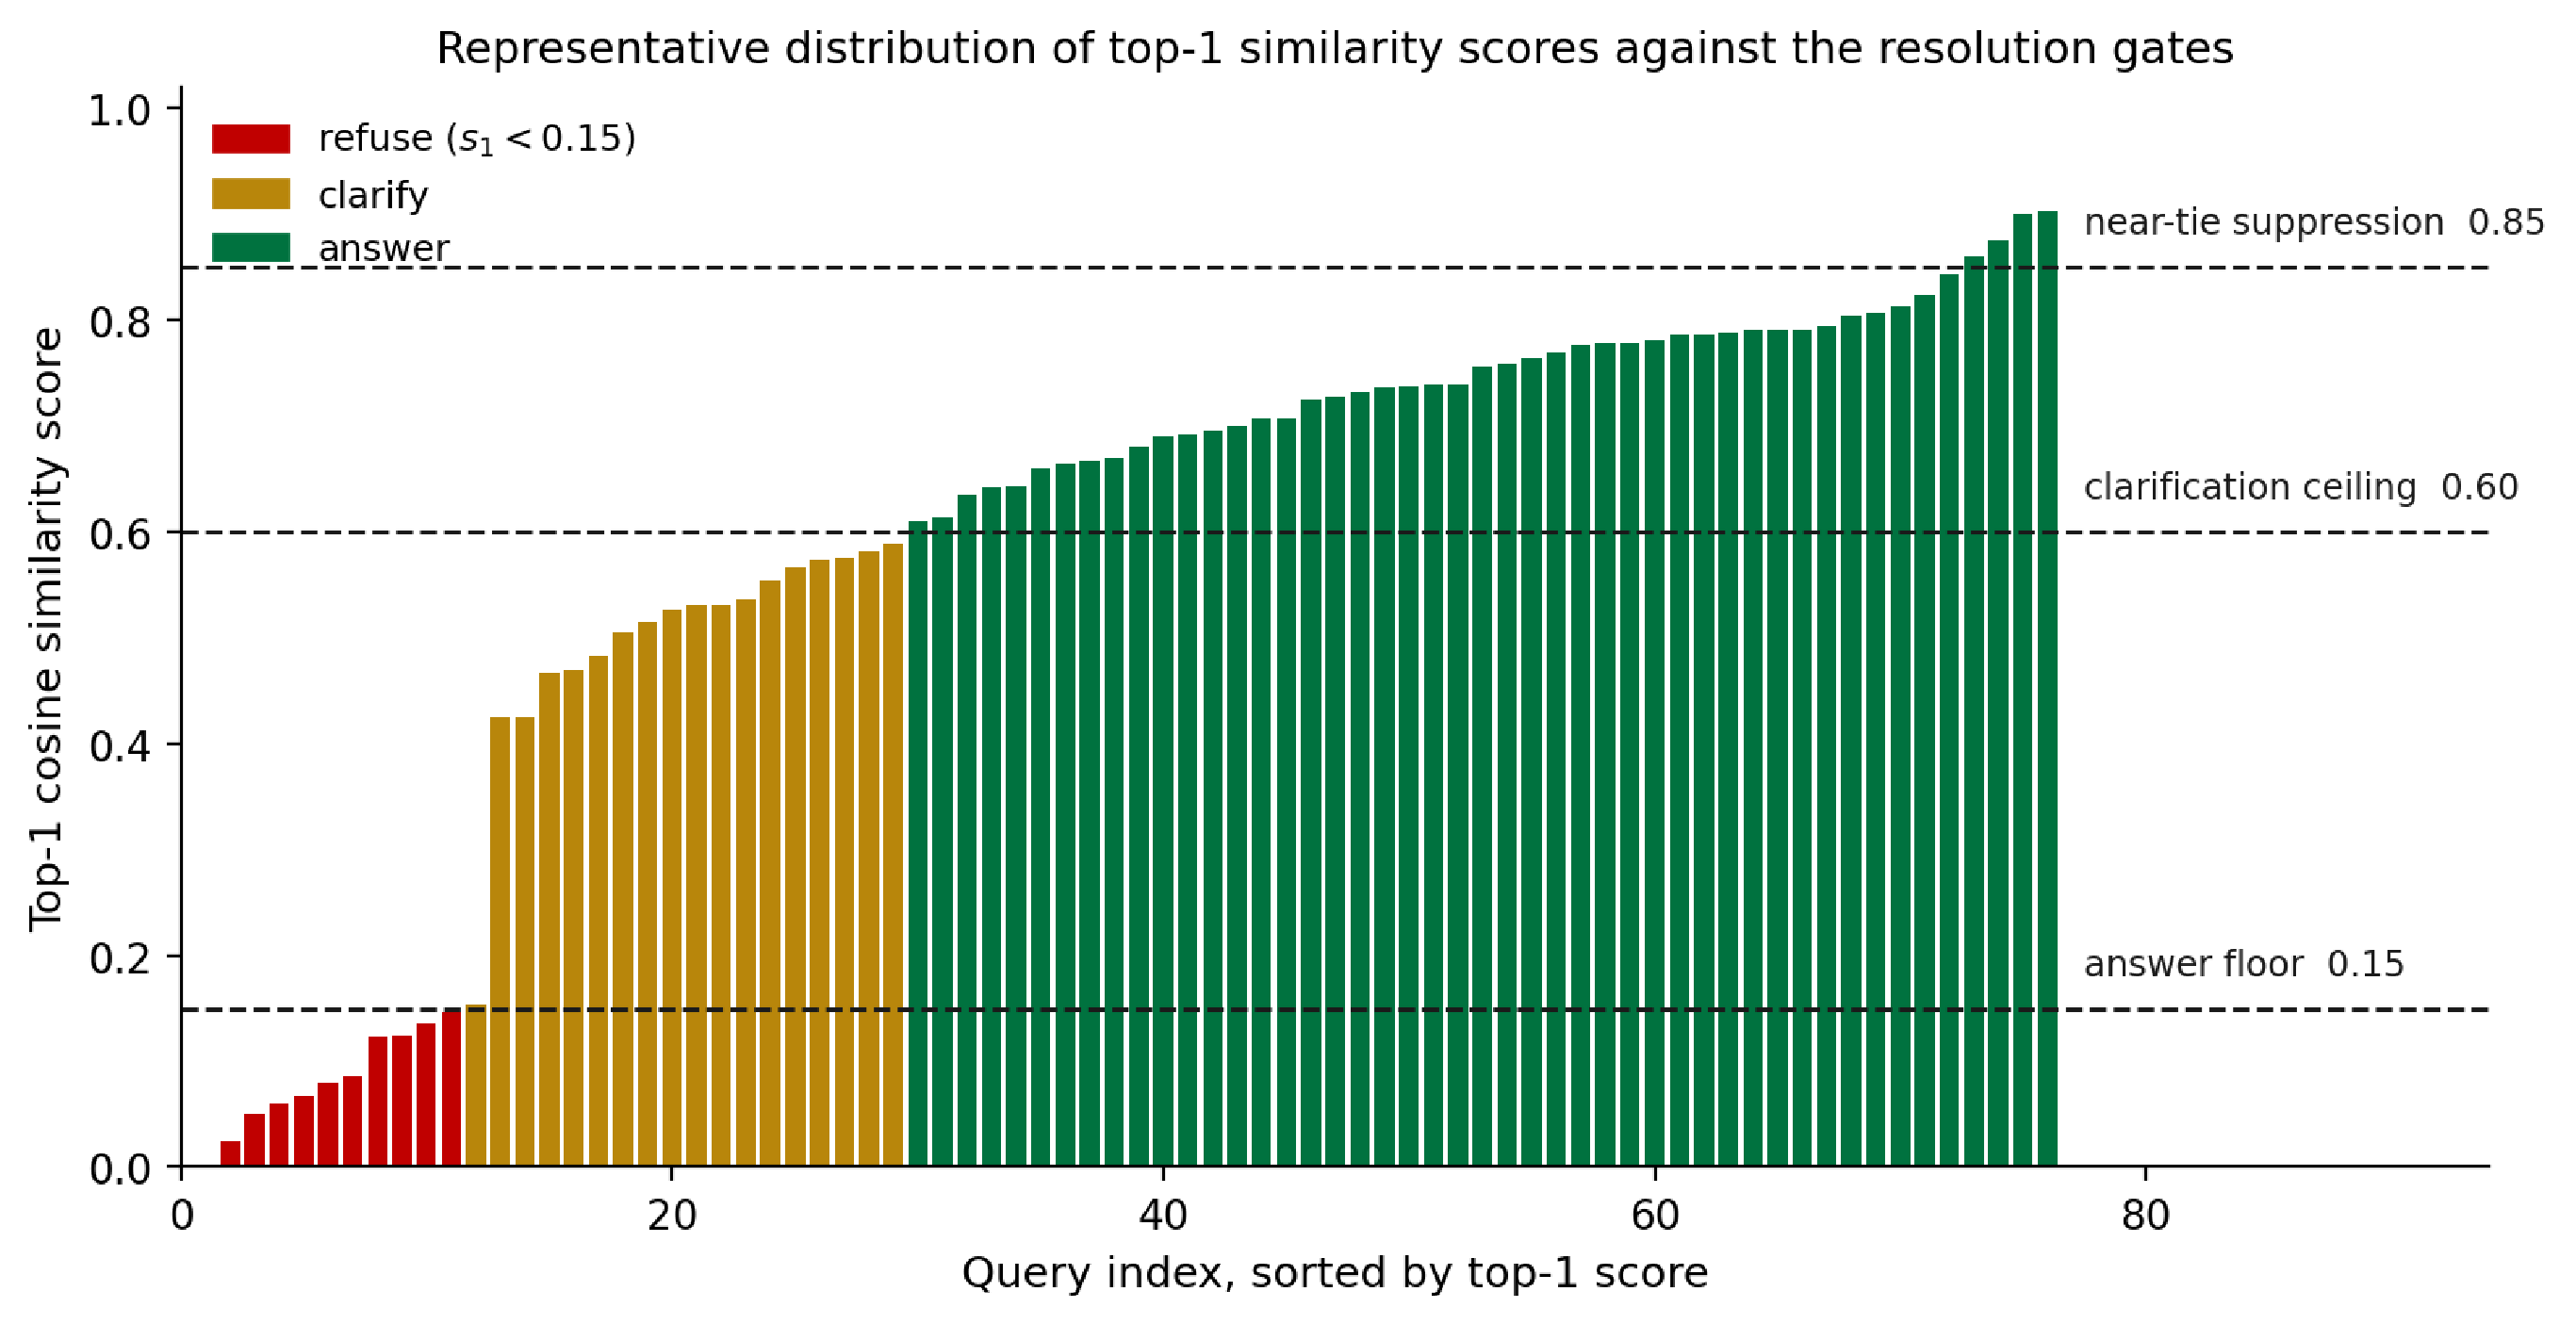
\includegraphics[width=0.9\textwidth]{figures/fig5_score_distribution.pdf}
\caption{Top-ranked similarity score across a batch of free-text queries, with the answer
floor, clarification ceiling, and near-tie suppression level marked.}
\label{fig:scoredist}
\end{figure}

Figure~\ref{fig:scoredist} places observed scores against these gates.

\section{Deterministic Answer Construction}

Once an activity has been resolved, the system still has to decide what the question was
actually asking about it, what else the document requires to be said regardless of the
question, and what to do when there is no honest answer to give.

\subsection{Intent Detection}

When the activity has been classified, the system then knows what kind of question is being asked about it. Questions are mapped to authority codes in the document, and the mapping needs to take into account how people ask these questions, with ``who signs off on this?'' meaning an approval and ``who has to check this?'' meaning check and verify.

This mapping cannot be naive when it comes to the letter C. According to Chapter~1, C1 and C2 are check and verify whereas C3 and C4 are consult, and mapping ``check'' to the letter C would be mixing up two different duties. This is why intent detection is against full codes and not their initial letter.

\subsection{Mandatory Obligation Surfacing}

Where an answer provides the response to the question, it also includes that which the document requires to be included. In the case of an action that has a check-and-verify entry in the DAM, that entry will appear even where the question pertained to the approval entry. The names of any informed individuals on record will appear.

This is because this is not an addition of contextual information. It is simply a required entry in the DAM, and it is someone new to the company asking the very specific question who will need the other three answers. This note is hidden only if it would repeat the answer provided.

\subsection{Cross-Reference Following}

Where a resolved activity has no responsibilities of its own but does carry a cross-reference, the system follows the reference and reports the target's responsibilities, stating that it has done so. This mirrors what a human reader does when a row tells them to look elsewhere, and it converts a dead end into an answer.

\subsection{Honest Refusal}

Three situations lead to a non-answer. In the case of an identifier that doesn't exist, the fact that it doesn't exist is stated, and a request is made to validate the identifier or describe what is happening. When a question is too vague to answer, the user is asked to provide additional information. When a question is off-topic, it is considered out of scope.

This is what should not happen in any of these scenarios. This is what requirement FR7 asks for and what makes positive answers valuable: a machine that knows all does not tell us anything about the reliability of its answers.

\section{Auxiliary Query Types}

But not all queries are authority queries. There are three more query types that get answers directly.

Glossary queries ask for the definition of an abbreviation and are answered using the abbreviations found in the document along with a small list of aliases for the acronyms found in role descriptions and not explicitly expanded. If the answer comes from the list of aliases, then the source of the definition is reported.

Authority-code queries ask for the definition of a code and are answered from the legend of the transcription. Authority codes detection is conservative on naked codes to avoid collision of 'I' with the pronoun. A naked code becomes a real mention only if it appears in the same sentence with some other code or is unambiguously used, like the parenthesized informed status marker or an alphanumeric combination not forming an English word.

Input queries are matched to anchored patterns and answered directly, bypassing the lookup pipeline. Patterns match anchored to the whole query string to avoid matching of 'hi' in the phrase 'history of the DAM'.

\section{Hybrid Language Model Layer}

Answer phrasing is delegated to a language model through a provider interface with two implementations and four operating modes.

\begin{longtable}{|p{0.16\textwidth}|p{0.30\textwidth}|p{0.44\textwidth}|}
\caption{Language model providers and operating modes.}\label{tab:llm}\\
\hline
\rowcolor{myblue}\textcolor{white}{\textbf{Mode}} & \textcolor{white}{\textbf{Provider}} & \textcolor{white}{\textbf{Behaviour}} \\
\hline
\endfirsthead
\hline
\rowcolor{myblue}\textcolor{white}{\textbf{Mode}} & \textcolor{white}{\textbf{Provider}} & \textcolor{white}{\textbf{Behaviour}} \\
\hline
\endhead
Auto & Cloud, falling back to local, then template & Default. Uses whichever provider is available, and the deterministic template if neither is. \\ \hline
Cloud & Groq\citep{groq} & Hosted inference. Fast, requires an API key and network access. \\ \hline
Local & Ollama\citep{ollama} & Runs on the same machine or in a companion container. No external dependency. \\ \hline
Off & None & Template answers only. Every lookup capability remains available. \\ \hline
\end{longtable}

It has been intentionally designed such that the agent and the providers interface is very small, and this has served to be of great benefit in the course of the project where a hosted model was deprecated by the provider and started throwing errors in the deployment environment. The solution was a mere modification of a constant behind the interface, without any impact on the agent and its tests.

\subsection{Model Configuration}
\label{sec:modelconfig}

Table~\ref{tab:models} records the models each mode resolves to and the task each performs.
Every identifier is read from configuration rather than compiled in, so a deprecated model
is replaced without a code change.

\begin{longtable}{|p{0.20\textwidth}|p{0.30\textwidth}|p{0.38\textwidth}|}
\caption{Models used by task, with the mode that selects each.}\label{tab:models}\\
\hline
\rowcolor{myblue}\textcolor{white}{\textbf{Task}} & \textcolor{white}{\textbf{Model}} & \textcolor{white}{\textbf{Notes}} \\
\hline
\endfirsthead
\hline
\rowcolor{myblue}\textcolor{white}{\textbf{Task}} & \textcolor{white}{\textbf{Model}} & \textcolor{white}{\textbf{Notes}} \\
\hline
\endhead
Answer phrasing, hosted & \texttt{openai/gpt-oss-120b} & Default for the hosted mode. Reached over an OpenAI-compatible chat completions interface. \\ \hline
Answer phrasing, local & \texttt{llama3.1} & Default for the local mode, served on \texttt{localhost:11434}. Selected when no hosted credential is present and the local service answers. \\ \hline
Transcription & \texttt{whisper-large-v3-turbo} & Converts a dictated audio clip to text. Hosted only; the local mode has no transcription path. \\ \hline
Image understanding & \texttt{qwen/qwen3.8-27b} & Used for image attachments. Requested through the same endpoint with an image content part carrying a base64 data URL. \\ \hline
Translation and tone & As answer phrasing & Both reuse whichever provider the active mode resolved to; neither has a model of its own. \\ \hline
\end{longtable}

Vision support is a property of the provider rather than of the mode. The provider interface
exposes a capability flag that is false by default and true only for the hosted provider, and
the attachment path tests that flag before constructing a request. An image sent while the
local mode is active is refused with a statement of the limitation rather than dispatched to
a model that would ignore it.

\subsection{Language Detection}
\label{sec:langdetect}

Translation is expensive relative to retrieval, so a deterministic pre-filter decides whether
the translation path runs at all. The filter uses three tests and returns true on the first
that matches: presence of any character in the Arabic block \texttt{U+0600}--\texttt{U+06FF};
presence of an accented Latin character from the set
\texttt{àâäéèêëïîôöùûüçñãõ}; or a whole-word match against per-language function-word lists
holding French, Spanish and Portuguese closed-class terms.

A single function-word hit is sufficient. The threshold is set there because a realistic
short question contains very few of them once domain vocabulary is excluded: the French
phrasing of ``who approves 3.111'' contributes exactly one, namely \emph{qui}. Requiring two
hits fails on that query.

Setting the bar that low is only safe because of what a false positive costs. A query wrongly
flagged as non-English is sent through translation, and the model reports the language as
English and returns the text unchanged, so the cost is one additional round trip and never an
altered answer. The word lists were also screened against ordinary English DAM vocabulary,
and ambiguous single-letter entries were removed for the same reason.

Retrieval itself is never multilingual. A non-English question is translated into English
before it reaches the index, and the answer is translated back afterwards, so the index, the
correction vocabulary, and the thresholds in Table~\ref{tab:thresholds} operate on English in
every case and behave identically regardless of the language the user typed.

\section{Grounded Generation and the Verification Check}

The facts are settled by this point; what remains is turning them into readable prose
without letting the model that does the wording quietly change what was said.

\subsection{Contract Given to the Model}

This model has no access to the knowledge graph and does not make decisions about what to retrieve. It gets a question, some set of previously retrieved facts, and a system prompt asking it to express these facts naturally without fabricating anything, omitting anything, and using any formatting. In case when the answer needs to be formulated in another language, there is an additional rule for the model that instructs it to translate the sentence without changing role names, identifiers, and footnotes.

Figure~\ref{fig:grounding} traces the complete flow, and the position of the verification step in it is the point of the diagram: the model sits inside the loop, not at its end, and nothing it produces reaches the user without being checked back against the facts it was given.

\begin{figure}[htbp]
\centering
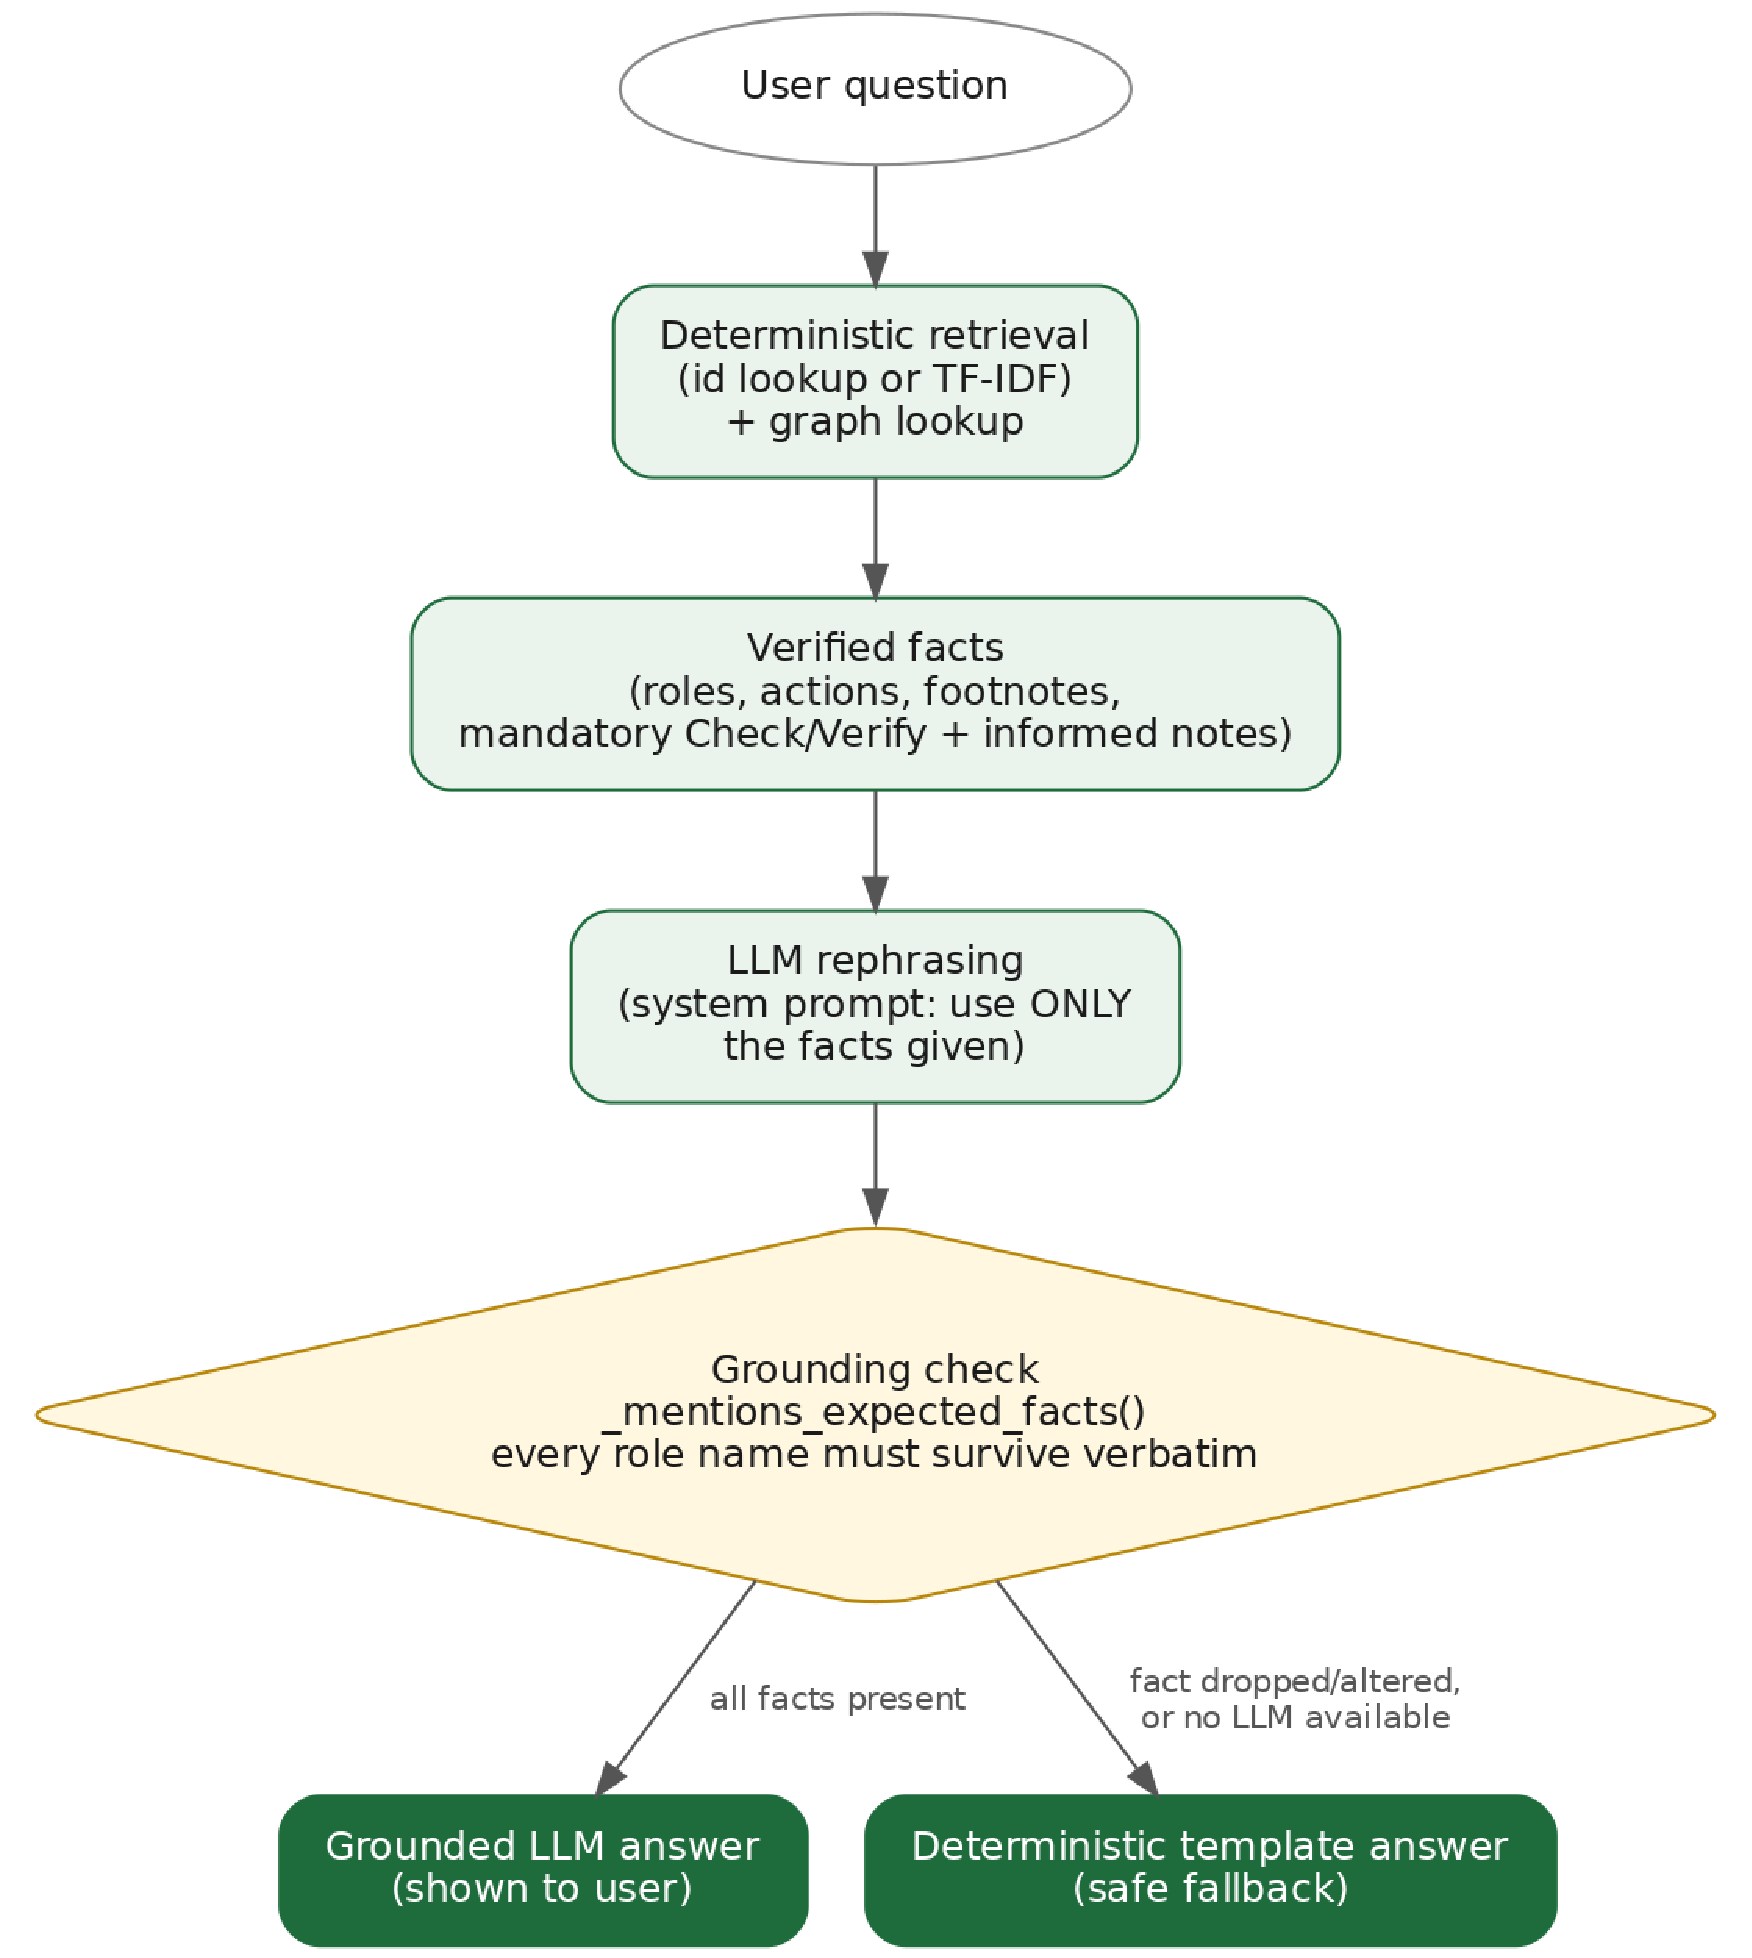
\includegraphics[width=0.94\textwidth,height=0.88\textheight,keepaspectratio]{figures/fig4_grounding.pdf}
\caption{Grounded generation flow. The model may only rephrase facts that have already been verified, and any rephrasing that drops or alters a fact is discarded in favour of the deterministic template answer.}
\label{fig:grounding}
\end{figure}

\subsection{Verification Step}
\label{sec:verification}

The instruction is a prompt, but not a guarantee. The verification converts the instruction into a property of the system.

Before the answer is generated, it is verified whether any role mentioned in the list of facts that back up the answer is found in the generated answer. In case of the absence of any of them, the generated answer is dropped, and a deterministic template answer is provided instead. The verification process relies on the containment test and not on the similarity test. Therefore, the paraphrasing of a role would not pass verification. The instruction that renamed, combined two roles into one or omitted the third role out of four informed people failed to satisfy the verification criterion regardless of fluency.

For both sides of comparison normalization of whitespace and case was applied. The reason for this tolerance was the fact that the previous version of verification used to fail some otherwise correct answers owing to mere formatting differences. The adjustment made the process less sensitive to formatting without reducing the correctness of verification, as all the same words in the same order should be present anyway.

\subsection{Answer Length and the Fallback Rate}

At first, the verification process happened more often than expected. The reason for that turned out to be a conflict between two instructions rather than the lack of reliability of the model. The instruction included in the system prompt dictated the answer containing from one to three sentences. It is impossible to articulate all duties of some activities in three sentences; hence, the model did not include some facts in accordance with the brevity instruction, and the verification was right.

The correction involved loosening the brevity condition rather than the accuracy condition. In case the number of facts backing up an answer exceeded a certain threshold, the brevity instruction was replaced by another instructing to use as many sentences as needed to cover the facts, while other constraints should stay in effect.

\section{Conversational Capabilities}

A single-turn question-answer exchange covers most of what earlier sections describe, but a
conversation is rarely that tidy in practice. The capabilities layered on top of single-turn
resolution include carrying the subject across a follow-up, adapting tone, handling
multilingual phrasing, and working from a worked example rather than a bare identifier.

\subsection{Context Carry-Over}

A user who has just asked about an activity and then asks ``and who has to be informed?''
expects the second question to be understood against the first. The client passes the
identifier resolved by the previous exchange back to the server as
\texttt{previous\_node\_id} on each subsequent request, and where a follow-up contains no
resolvable subject of its own, the retrieval layer answers it against that identifier
rather than returning a failure. The interface then states explicitly that the subject was
carried over, so that a user is never left to infer which activity an answer refers to.

Carry-over is state held by the client rather than by the server. The server remains
stateless with respect to conversational context: it is told the previous identifier on
each call instead of remembering it, which keeps a conversation reproducible from its
transcript alone and avoids any session affinity in deployment.

The mechanism required an explicit suppression rule. Carry-over was initially applied
whenever a question failed to resolve a subject, which silently captured question types
that have nothing to do with the previous activity. Asking what an authority code means
while an activity was in context produced an answer about that activity rather than about
the code, because the code question resolved no subject of its own and was therefore
treated as a follow-up. Auxiliary query types, glossary lookups, authority-code
explanations and small talk, are now classified before carry-over is considered, and are
excluded from it.

\subsection{Tone Adaptation}

Questions are classified as neutral, frustrated, or confused, and a short empathetic
opener is prepended where the tone is not neutral. The classification is gated behind a
deterministic pre-filter: a lexical check for markers of frustration or confusion decides
whether a model call is worth making at all, so a neutral question, which is the
overwhelming majority of traffic, incurs no additional latency or cost. Tone is assessed
against the text the user actually typed rather than against any internally translated
version of it, since translation normalises register and would erase precisely the signal
being measured.

Tone affects only the opener. It cannot alter the facts that follow it, which are
assembled before tone is ever considered.

\subsection{Multilingual Questions}

Questions in French, Spanish, Portuguese, or Arabic are detected, translated into English
for retrieval, and answered in the language in which they were asked. Detection uses a
deterministic pre-filter over character ranges and function-word lists rather than a model
call, so an English question, again the common case, is never charged for a capability it
does not use.

Retrieval itself remains English-only and entirely unchanged. This is deliberate: the
index, the typo-correction dictionary and the identifier grammar are all built from the
document's own English vocabulary, and translating the question before retrieval rather
than localising the index means that the retrieval behaviour tested in this chapter is
exactly the behaviour a non-English user receives. Two distinct language concerns are
kept separate in the implementation, the language a question must be translated
\emph{from} for retrieval, and the language the answer is phrased \emph{in}, so that an
English question can be answered in French when the interface language has been set
explicitly.

The verification check described in Section~\ref{sec:verification} is not translated. It
continues to search for the literal English role names inside the generated answer
whatever language the surrounding sentence is written in. A French answer that has dropped
a role therefore fails exactly as an English one would, and the guarantee does not weaken
as language support widens.

\section{Worked Examples}

The following exchanges were run against the delivered build and are reproduced as the
system produced them.

Asking \textit{``who approves 2.126''} resolves by identifier with confidence 1.0 to the
quarterly mission programme activity, and names the Regional Director General and the
Director of the Nigeria office as approvers, with the abbreviation expanded inline. The
answer also states that the task must be checked and verified by the Sector Manager and
the Supporting Department Division Manager, and that the concerned Sector Vice-President,
the Regional Vice-President, and the Task Manager or Project Team must be informed. None
of that was asked for. All of it is mandatory, and surfacing it is the behaviour required
by FR4.

Asking \textit{``who needs to be informed for quarterly mission program''} resolves the
same activity from its name alone, through the lexical path rather than the identifier
path, with the answer now centred on the informed parties.

Asking \textit{``who aproves the qaurterly mision program''}, with three deliberate
misspellings, resolves identically. The correction is deterministic, so the behaviour is
identical with or without a model provider available.

Asking \textit{``who initiates 1.117.2''} exercises the redirect path. That activity's own
row records no responsibilities and points to another activity, so the system follows the
pointer and reports the target's responsibilities instead of dead-ending on an empty
record.

Asking \textit{``who approves of Communication with Co-Financiers of projects''} followed
by \textit{``and who are the informed parties?''} exercises carry-over: the second
question, which names no subject, stays on the activity resolved by the first.

Asking \textit{``what happens with 9.999.999''} produces a refusal, stating that the
identifier does not exist and suggesting that the user check it or describe the activity
in words. This is the behaviour the design exists to produce, and it is worth reading as a
result rather than as a limitation: the alternative, a plausible answer about a
neighbouring activity, is the failure mode this entire architecture was built to prevent.

\section*{Conclusion}
\addcontentsline{toc}{section}{Conclusion}

This chapter has described how a question becomes an answer. Resolution proceeds through
an identifier fast path and a lexical search layer, both deterministic, and answers are
constructed from records held in the knowledge graph rather than generated. A language
model participates only in how an answer reads, never in what it asserts, and a
verification step compares the generated text against the retrieved facts and discards any
rephrasing that has lost one of them.

The value of that separation is that it makes a guarantee possible. Retrieval may fail,
and when it does the system says so; but an answer that is returned cannot contain a role
or an obligation the document does not record, because no component downstream of
retrieval is permitted to introduce one. Around that core sit the behaviours that make the
system usable rather than merely correct: typo tolerance, redirect following, mandatory
obligation surfacing, context carry-over, tone adaptation, multilingual handling, and
explicit refusal.

What this chapter has not addressed is everything surrounding the agent: who is allowed to
use it, how conversations persist, how answers reach a user who is not at a keyboard, and
what the accumulated structure of the matrix itself reveals when it is examined in
aggregate. The next chapter presents the platform built to deliver those.
